%!TEX output_directory = latex_out/

\documentclass[12pt]{article}
\usepackage[letterpaper, margin=1in, headheight=15pt]{geometry}
\usepackage{amsmath}
\usepackage{setspace}
\usepackage{pgfplots}
\usepackage{fancyhdr}
\usepackage{csquotes}
\usepackage{todonotes}
\usepackage{verbatim}
\usepackage[toc]{appendix}
\usepackage[natbibapa]{apacite}

% set up PGF
\pgfplotsset{compat=1.6}
\newcommand\inputpgf[2]{{
\let\pgfimageWithoutPath\pgfimage
\renewcommand{\pgfimage}[2][]{\pgfimageWithoutPath[##1]{#1/##2}}
\input{#1/#2}
}}

% set up notes-- different backgrounds for Nolan and Joe!
\newcommand\nbcnote[1]{\todo[inline, backgroundcolor = yellow]{\textbf{NBC}: #1}}
\newcommand\jlanote[1]{\todo[inline, backgroundcolor = lime]{\textbf{JLA}: #1}}

% set up header % 
\pagestyle{fancy}
\fancyhf{} % sets both header and footer to nothing
\renewcommand{\headrulewidth}{0pt}
\lhead{RUNNING HEAD: Similarity and Contrast in Concept Generation}
\fancyhead[R]{\thepage}


\begin{document}
\doublespacing


% \documentclass[12pt]{article} \usepackage[letterpaper, margin=1in, %
%headheight=15pt]{geometry} \usepackage{amsmath, listings}


% \begin{document}
\section{Experiment 3}

Experiments 1 and 2 clearly establish the importance of contrast in category
generation. Follow-up model-based analyses illustrated that both contrast models
account for participant performance better than models that do not take into
account contrast. We also found more support for contrast as representativeness
hypothesis over contrast as exemplar dissimilarity hypothesis.

Although category generation is an intriguing aspect of human cognition, it has
played a relatively limited role in the broader categorization literature. To
establish that contrast plays a broader role in categorization, we conducted a
traditional category learning study. In it, participants learned two categories,
where the categories learned by each participant in Experiment 3 was yoked to
the Alpha shown and Beta generated by each participant in Experiment 2. Our goal
is to investigate whether model performance (in generating categories) is
consistent with human performance (in learning those categories). Specifically, if contrast plays a broader role in categorization, then Beta categories rated as "better" according
to the contrast models should be easier for participants to learn.
%\footnote{It is possible to adjust the present models of category generation such that they can make category learning predictions. However, such an adjustment makes the strong assumption that the very same processes governing category generation also apply to category learning. Taking this approach would fall outside the scope of the current investigation.} 
\subsection{Participants, Materials, and Procedure}

Experiment 2 recruited 122 participants who each generated one set of four Alpha
and four Beta category exemplars. Experiment 3 recruited the same number of
participants.

Participants observed four blocks of eight trials. Each trial began with the
presentation of a fixation cross for 500 ms. This was followed by the
presentation of one exemplar randomly sampled without replacement from the
unique category set. Participants were tasked with assigning the presented
exemplar to either the Alpha or Beta category with no time limit imposed.
Feedback was automatically displayed for 2500 ms after each response.

\subsection{Results and Analysis}

Among the 122 originally generated category sets were 102 unique sets (i.e.,
they contained a unique collection of Alpha and Beta exemplars). Consequently,
for our subsequent analyses for this experiment we only use data from the first
102 participants that were presented with a unique category set.

Overall accuracy of the participants was high, with a mean error rate of $.19$
($SD = .19$). Aggregated error rates for each block are presented in Figure
\ref{fig:learningcurve}.

\begin{figure}
    \begin{center}
    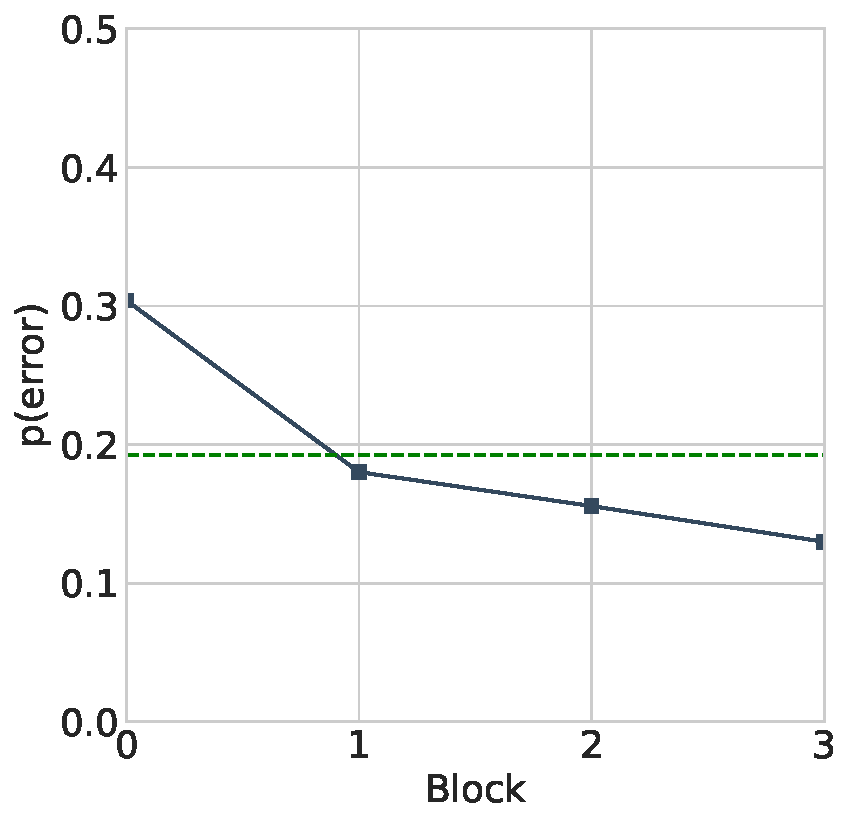
\includegraphics[width=\textwidth/2]{figs/e3-learningcurve.pdf}
    \caption{Average error rate for each successive block. Green discontinuous
line represents the overall mean error rate.}
    \label{fig:learningcurve}
    \end{center}
\end{figure}

In order to analyze the consistency between model and human performance, we
optimized each model such that the Pearson correlation between the model's
negative log-likelihood of generating each unique category set and the
participant's error in learning that category set is maximized. As with the
analysis in Section \ref{section:individual-diff}, we simulated the weighting of
each dimension independently depending on the generated categories.

The greatest correlations were observed when fitting with the contrast models.
Specifically, PACKER correlated with human performance with
$r = .65, 95\% CI$\footnote{Confidence intervals were obtained using a bootstrap
  method with 1000 bootstrap samples.}$ [.48,.78]$, and the representativeness
model correlated with human performance with $r = .59, 95\% CI [.40, .73]$.
Copy-and-tweak yielded a correlation of $r = .45, 95\% CI [.28, .62]$ and the
hierarchical Bayesian model yielded a similar correlation of
$r = .46, 95\% CI [.30, .62]$. These results are graphically presented in Figure
\ref{fig:perror_corr}.

\begin{figure}
    \begin{center}
    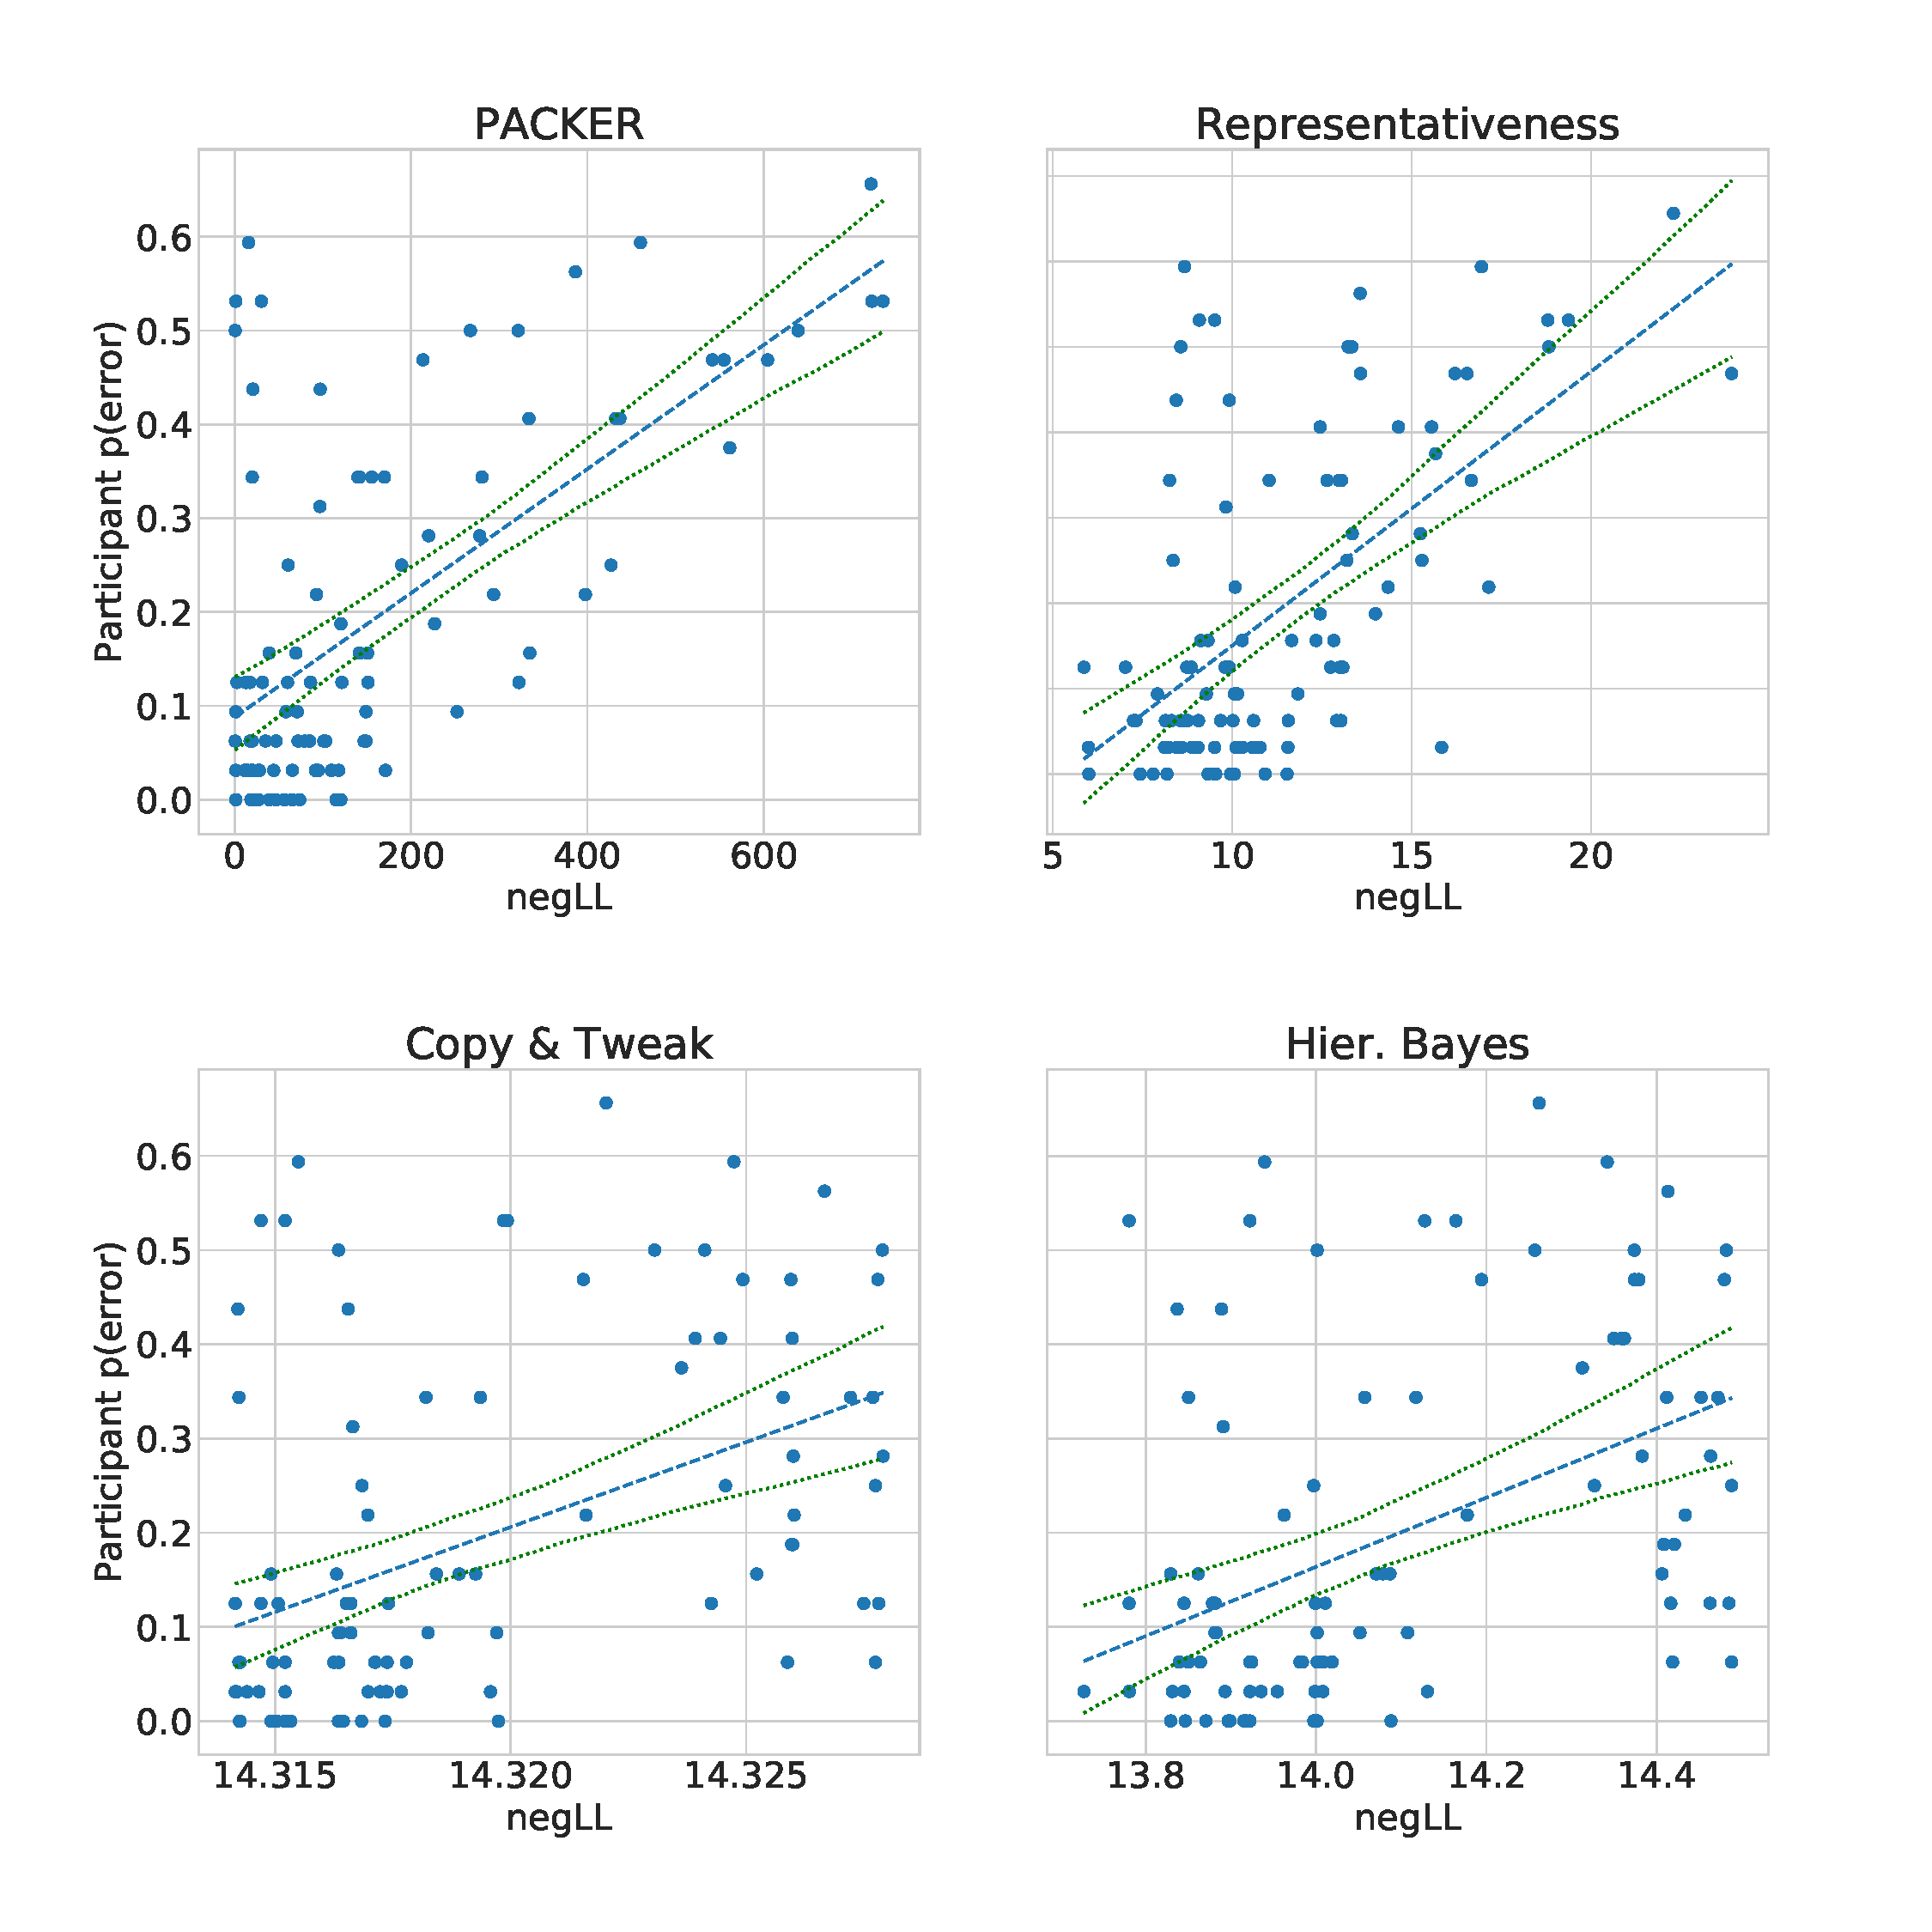
\includegraphics[width=\textwidth]{figs/modelvspptp.pdf}
    \caption{Scatterplots indicating the correlations between observed
      participant error and model fit. Blue discontinuous line are best-fit
      lines. Green discontinuous lines indicate boundaries generated by the 95\%
      CI around the fitted correlations. }
    \label{fig:perror_corr}
    \end{center}
\end{figure}

To emphasize the strong influence of contrast in maximizing the association
between category generation and category learning, we computed the correlations
over wide range of $\theta_{contrast}$ values, with the other parameter values
of PACKER held constant at their optimized levels. As presented in Figure
\ref{fig:packer-corr}, the correlation quickly increases with increasing weight
on contrast, reaching a plateau above values of around 4.0.

\begin{figure}
    \begin{center}
    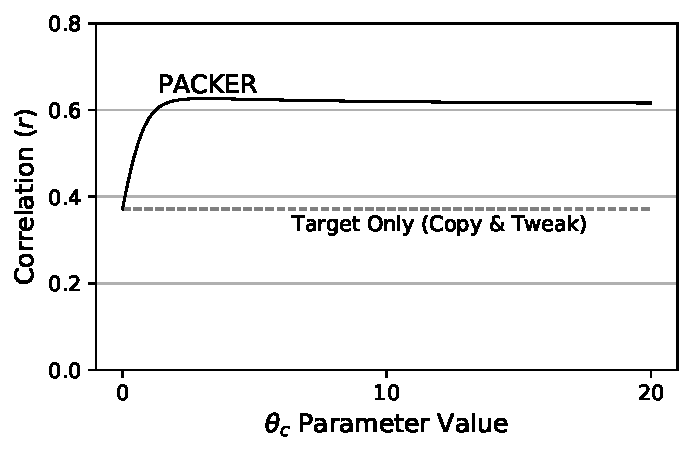
\includegraphics[width=0.8\textwidth]{figs/packer-corr.pdf}
    \caption{Correlation between PACKER's fit and participant error as a
function of the $\theta_{contrast}$ parameter. To facilitate comparison,
PACKER's other parameters ($c$, $\theta_{target}$) were set to the best fitting
values obtained for copy-and-tweak in Table \ref{table:global-model-fits}. Grey
dashed line represents the correlation between Copy \& Tweak's fit and
participant error.}
    \label{fig:packer-corr}
    \end{center}
\end{figure}


\end{document}
